
TypeScript --- язык программирования с открытым исходным кодом, разрабатываемый и поддерживаемый Microsoft Corporation. Является более строгим надмножеством языка JavaScript
и добавляет опциональные элементы статической типизации и основанную на механизме классов (в отличие от механизма прототипов для Native JavaScript) реализацию объектно-ориентированной парадигмы.
Данный язык, являясь надстройкой над JS, может использоваться для разработки как клиентских приложений для выполнения в браузере, так и серверных для выполнения в таких средах,
как Node.js или JSX. \cite{typescript1}\cite{typescript2}

Среди основных отличий языка от Native JavaScript можно отметить следующие особенности:
\begin{itemize}
\item типовые аннотации для функций и членов классов;
\item файлы объявлений;
\item классы и интерфейсы;
\item generic-типы;
\item модули и пространства имен;
\item смешения (Mixin);
\item типы-перечисления;
\item инструкция \textit{await};
\item кортежи.
\end{itemize}

Основное назначение языка - упрощение разработки более крупных клиентских приложений, добавление механизмов статической типизации, позволяющих избежать большого количества
простых ошибок на этапе транскомпиляции, которые могли бы повлиять на выполнение кода во время работы программы. Тем не менее, поскольку статическая типизация является
опциональной (однако, ее можно установить принудительно посредством некоторых флагов компиляции, таких как --noImplicitAny), все программы, написанные на Native JavaScript,
также являются валидными TypeScript программами. Это обеспечивает обратную совместимость и простую миграцию для legacy-проектов. Разработчики TypeScript искали решение,
которое не будет нарушать совместимость со стандартом и его кросс-платформенной поддержкой. Зная, что только стандарт ECMAScript\cite{ECMAScript}\cite{ECMAScript2} предлагает поддержку в будущем для
программирования на базе классов (Class-based programming), TypeScript был основан на этом предположении. Это привело к созданию компилятора JavaScript с набором
синтаксических языковых расширений, увеличенным на основе предложения, которое трансформирует расширения в JavaScript. В этом смысле TypeScript является представлением
того, что ожидать от ECMAScript 6 (рисунок \ref{fig:theory:typescript:typescript}). Уникальный аспект не в предложении, а в добавлении в TypeScript статической типизации,
что позволяет статически анализировать язык, облегчая оснастки и IDE поддержку.

\begin{figure}[ht]
\centering
  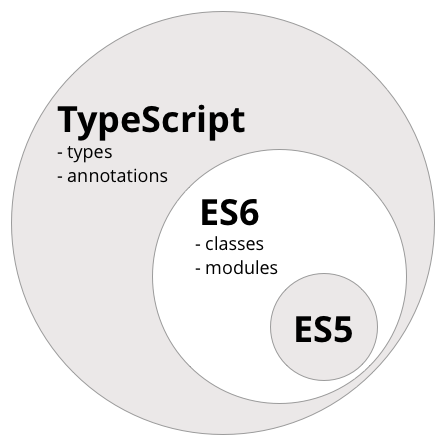
\includegraphics[scale=0.75]{typescript.png}
  \caption{Функционал языка TypeScript}
  \label{fig:theory:typescript:typescript}
\end{figure}

Одним из результатов работы TypeScript компилятора является набор так называемых typing-файлов, имеющих расширение *.d.ts. Данные файлы - вспомогательные для
компилятора и являются метаданными модулей и классов, компилируемых TypeScript. Ближайшим аналогом данных файлов являются *.h и *.hpp файлы языков C/C++. Данные
typing-файлы хранят информацию о публичном интерфейсе генерируемых классов и являются <<клеем>>, связывающим сгенерированные *.js файлы с исходными *.ts и *.tsx файлами.

Статический анализ typing-файлов позволяет реализовать механизм подсказок и автодополнение кода в IDE, поддерживающих TypeScript. Среди самых распространенных
можно отметить следующие IDE:
\begin{itemize}
\item Atom Text Editor с плагином Typed --- основной текстовый редактор, используемый в данной дипломной работе;
\item Visual Studio 2013 Update 2 и позже;
\item GNU Emacs с плагином <<Company>>.
\end{itemize}

Для автоматизации процесса транскомпиляции TypeScript целесообразно использовать так называемые <<Task-runner>> программы, такие как <<Grunt>> или <<Gulp>>.
Использование оных позволяет подписаться на события изменения файлов исходного кода проекта и перекомпилировать проект в JavaScript по мере изменения исходного
кода в автоматическом режиме. Для настройки данных инструментов используются Gruntfile либо Gulpfile (в зависимости от избранного Task-runner). Эти файлы,
являясь аналогами GNU Makefile, есть ни что иное как скрипты для компиляции, определяющие конвеер, обрабатывающий все файлы в проекте по мере их модификации.
Реализация данных файлов на ранних этапах разработки проекта позволяет повысить степени автоматизации и легко внедрить такие инструменты разработки, как
средства продолжительной интеграции, автоматизированное тестирование и версионирование исходного кода.
